
\section{Overview of VQE} \label{sec:overview}

In this section, we aim to provide sufficient information for our reader to acquire a technical understanding of the VQE, and an appreciation of where the algorithm is positioned compared to both conventional electronic structure, and other quantum methods. We also provide an outline for the suggested best practices, collected from the remainder of the review, and a perspective on the overall resources that could be required for the VQE to achieve quantum advantage.

\subsection{A formal definition of the VQE}

The VQE was first presented in Ref. \cite{Peruzzo2014} and its theoretical framework was significantly extended in Ref. \cite{mccleanTheoryVariationalHybrid2015}. It is grounded in the variational principle (and more precisely in the Rayliegh-Ritz functional \cite{Rayleigh1870, Ritz1908, Arfken1985}), which optimizes an upper bound for the lowest possible expectation value of an observable with respect to a trial wavefunction. Namely, providing a Hamiltonian $\hat{H}$, and a trial wavefunction $\ket{\psi}$, the ground state energy associated with this Hamiltonian, $E_0$, is bounded by
\begin{equation}
    E_0 \leqslant \frac{\bra{\psi}\hat{H}\ket{\psi}}{\braket{\psi | \psi}}. \label{eq:ritzfunc}
\end{equation}
The objective of the VQE is therefore to find a parameterization of $\ket{\psi}$, such that the expectation value of the Hamiltonian is minimized. This expectation value forms an upper bound for the ground state energy, and in an ideal case should be indistinguishable from it to the level of precision desired. In mathematical terms, we aim to find an approximation to the eigenvector $\ket{\psi}$ of the Hermitian operator $\hat{H}$ corresponding to the lowest eigenvalue, $E_0$.

In order to translate this minimization task into a problem that can be executed on a quantum computer, one must start by defining a so-called ansatz wavefunction that can be implemented on a quantum device as a series of quantum gates. Given that we can only perform unitary operations or measurements on a quantum computer, we do this by using parametrized unitary operations (see Sec. \ref{sec:Ansatz}). We hence express $\ket{\psi}$ as the application of a generic parametrized unitary $U(\boldsymbol{\theta})$ to an initial state for $N$ qubits, with $\boldsymbol{\theta}$ denoting a set of parameters taking values in $(-\pi, \pi]$. The qubit register is generally initialized as $\ket{0}^{\otimes N}$, written as $\ket{\boldsymbol{0}}$ for simplicity, although low-depth operations can be performed for alternative initializations before the unitary is applied. Noting that $\ket{\psi}$ (as well as any $U(\boldsymbol{\theta}) \ket{\psi}$) is necessarily a normalized wavefunction, we can now write the VQE optimization problem as
\begin{equation} \label{eq:vqe_cost_function}
    E_{\mathrm{VQE}} = \min_{\boldsymbol{\theta}} \bra{\boldsymbol{0}} U^{\dagger}(\boldsymbol{\theta})\hat{H}  U(\boldsymbol{\theta}) \ket{\boldsymbol{0}}.
\end{equation}
Eq.~(\ref{eq:vqe_cost_function}) is also referred to as the cost function of the VQE optimization problem, which is a terminology inherited from the machine learning and optimization literature. 
We can continue this description by writing the Hamiltonian in a form that is directly measurable on a quantum computer, as a weighted sum of spin operators (Sec. \ref{sec:Hamiltonian_representation} shows how the Hamiltonian can be defined, and Sec. \ref{sec:Encoding} how it can be mapped to spin operators). Observables suitable for direct measurement on a quantum device are tensor products of spin operators (Pauli operators). We can define these as Pauli strings: $\hat{P_{a}} \in \{I, X, Y, Z\}^{\otimes N}$, with $N$ the number of qubits used to model the wavefunction. The Hamiltonian can be rewritten as
\begin{equation}
    \hat{H} = \sum_{a}^{\mathcal{P}} w_{a} \hat{P}_{a},
\end{equation}
with $w_a$ a set of weights, and $\mathcal{P}$ the number of Pauli strings in the Hamiltonian. Eq.~(\ref{eq:vqe_cost_function}) becomes
\begin{equation} \label{eq:vqe_hybrid_function}
    E_{\mathrm{VQE}} = \min_{\boldsymbol{\theta}} \sum_a^{\mathcal{P}} w_a \bra{\boldsymbol{0}} U^{\dagger}(\boldsymbol{\theta})\hat{P}_{a}  U(\boldsymbol{\theta}) \ket{\boldsymbol{0}},
\end{equation}
where the hybrid nature of the VQE becomes clearly apparent: each term $E_{P_a} = \bra{\boldsymbol{0}} U^{\dagger}(\boldsymbol{\theta})\hat{P}_{a}  U(\boldsymbol{\theta}) \ket{\boldsymbol{0}}$ corresponds to the expectation value of a Pauli string $\hat{P}_a$ and can be computed on a quantum device, while the summation and minimization $E_{VQE} = \min_{\boldsymbol{\theta}} \sum_a w_a E_{P_a}$ is computed on a conventional computer.

\subsection{The VQE pipeline}

The VQE, as presented using Eq.~(\ref{eq:vqe_hybrid_function}), can be decomposed into a number of components, which all entail significant choices that impact the design and overall cost of the algorithm. We refer to the layering of these different components as the VQE pipeline. Most choices made on specific elements of this pipeline have significant implications on the entire VQE process. We summarize the iterative process (and the main VQE loop) in Fig. \ref{fig:VQE_pipeline} to provide a schematic visual description of the algorithm and its main components. We list the key components below and provide a brief introduction to each of them and how they fit together:

\begin{itemize}
    \item \textbf{Hamiltonian construction and representation:} The first step in the VQE is to define the system for which we want to find the ground state. This can be an \textit{ab initio} molecular Hamiltonian for electronic structure \cite{Parr1990, Friesner2005, Szabo1996, Jensen2017}, a solid-state system \cite{nemoshkalenko1998computational, Martin2004, Marder2010, Continentino2021}, a spin lattice model \cite{Clark1997}, a nuclear structure problem Hamiltonian \cite{Romero2022}, or a Hamiltonian describing any other quantum system. For each of these, one starts with a specific geometry (or conformation) of the system, specifying for example the distance between each atom, or the geometry of the lattice. Constructing the Hamiltonian involves finding specific operators and their weights between basis functions spanning the physical problem, where the basis functions represent the individual single-particle degrees of freedom. Given the Hamiltonian defines the quantum observable for the total energy associated with a wavefunction, the choice of basis is critical to define the space its spans. It can have a significant impact on the accuracy and cost of the final result, as the type of basis and number of basis functions chosen both determine the size of the computation required and the accuracy of the representation. %Furthermore, the ground state energy is in principle invariant to single-particle unitary transformations between these basis functions in which the system Hamiltonian is represented. This allows these degrees of freedom defining the basis to be unitarily rotated among each other, with the total energy remaining invariant to this operation. 
    In the case of electronic structure, these different representations could include, as examples, molecular orbitals from a prior mean-field calculation, plane-wave functions, or local atomic functions, all representing the spatial distributions (or `orbitals') for the single-particle Fock states, from which the many-body basis is formed \cite{Szabo1996}. 
    Additional complexity arises when specifically looking at electrons: following the Pauli exclusion principle \cite{Pauli1925, griffiths2005introduction} the wavefunction must be antisymmetric with respect to the exchange of two electrons. From a mathematical perspective, this means that we must decide whether we enforce this antisymmetry through the definition of the wavefunction or through the definition of the operators. These are referred to (for historical reasons) respectively as first and second quantization \cite{Szabo1996}.
    %In first quantization, Hamiltonian operators are simple projectors onto the basis chosen as all the complexity of maintaining the antisymmetry relation is constructed in the wavefunction. 
    In second quantization the Hamiltonian is expressed in terms of fermionic operators, also known as creation ($\hat{a}^{\dagger}_j$) and annihilation ($\hat{a}_j$) operators. These correspond to the action of adding, or removing an electron from a given basis function with integer index $j$, respectively (e.g. an orbital or a lattice site), ensuring appropriate fermionic antisymmetry with respect to permutation of any two particles. We provide an introduction to Hamiltonian construction and discuss the wider implications of particular representation choices in Sec. \ref{sec:Hamiltonian_representation}.
    \item \textbf{Encoding of operators:} Qubit registers on quantum computers can only measure observables expressed in a Pauli basis, due to the two-level nature of spins: $\hat{P_{a}} \in \{I, X, Y, Z\}^{\otimes N}$, for $N$ qubits. In first quantization, the operators can be directly translated into spin operators that can be measured on quantum computers \cite{mcardleQuantumComputationalChemistry2018}, as they are not used to enforce antisymmetry of the wavefunction - we briefly outline how this is done in Sec. \ref{sec:first_quantization}. In second quantization the Hamiltonian is expressed as a linear combination of fermionic operators which are defined to obey this antisymmetry relationship, unlike Pauli operators. The role of a fermionic to spin encoding is therefore to construct observables, from Pauli operators, which maintain this relationship. A transformation of fermionic operators to spin operators that meets this criterion was demonstrated a long time ago \cite{Jordan1928}, and recent research has focused on improving on this initial work. The key factors determining the efficiency of an encoding are their Pauli weight (the maximum number of non-identity elements in a given spin operator), the number of qubits required, and the number of Pauli strings produced. We provide a list of the most relevant encodings for second quantized Hamiltonians in Sec. \ref{sec:Encoding}. It is worth noting that for certain ansatz choices, in particular those defined in terms of fermionic operators, the encoding can have significant implications on gate depth and trainability (Sec. \ref{sec:Ansatz}). Cases of encoding particles others than fermions (e.g. bosons), and which do not require antisymmetry to be enforced are far simpler and are presented directly with the relevant Hamiltonian representation in Sec. \ref{sec:Hamiltonian_representation}. 
    \item \textbf{Measurement strategy and grouping:} The next step in the VQE pipeline is to determine how measurements are distributed and organized to efficiently extract the required expectation values from the trial wave function. In general, to achieve a precision of $\epsilon$ on the expectation value of an operator, we are required to perform $\mathcal{O}(1/\epsilon^2)$ repetitions (usually denoted as shots) of the circuit execution, each completed with a measurement at the end \cite{mccleanTheoryVariationalHybrid2015}. The objective of the measurement strategy is to make the number of repetitions as low as possible. Several techniques are available to achieve this, in particular, the use of efficient weighting of the number of measurements across the operators \cite{Wecker2015, Rubin2018, Arrasmith2020}. This can be further optimized by using properties of the Lie algebra in which Pauli strings are defined. \textit{Via} processing of the encoded Pauli strings to be measured, it is possible to identify commuting groups of operators that can be measured jointly, and subsequently find the measurement bases in which all operators of a given group can be simultaneously measured \cite{Gokhale2019_long, Hamamura2020, Huggins2021} (see Sec.~\ref{sec:discussion_grouping}). In order to perform this joint measurement, a short quantum circuit must therefore be designed and applied for each group, to rotate the measurement basis and to perform this joint measurement. Alternatively, because of information overlap between different Pauli strings, one can also try to reduce the number of measurements required using inference methods from fewer shots \cite{Torlai2020, Huang2020}, with further details in Sec.~\ref{sec:Grouping}.
    \item \textbf{Ansatz and state preparation:} Once the Hamiltonian has been prepared such that its expectation value can be measured on a quantum device, we can turn to the preparation of the trial wavefunction. In order to do this, one must decide on a structure for the parametrized quantum circuit, denoted as ansatz. It is used to produce the trial state, with which the Hamiltonian can be measured. Upon successful optimization of the ansatz parameters, the trial state becomes a model for the ground state wavefunction of the system studied. A wide range of ans{\"{a}}tze are possible, and the appropriate choice depends on the problem being addressed. The key aspects of the ansatz are its expressibility and trainability. The expressibility defines the ability of the ansatz to span a large class of states in the Hilbert space \cite{Holmes2021, Nakaji2021}, defining the maximum accuracy its approximation of relevant low-energy states can achieve (assuming all parameters can be perfectly optimized). Its trainability describes the practical ability of the ansatz to be optimized using techniques tractable on quantum devices \cite{Cerezo2021_BP, Holmes2021} (related to the total number of parameters, their linear dependence, the structure of the optimization surface, and to the related concept of barren plateaus \cite{McClean2018}, which can arise when gradients almost vanish thereby preventing optimization). A good ansatz must be sufficiently expressive to guarantee that it can appropriately approximate the ground state wave function, however, it must not be so expressive that it renders the search for the target state intractable. Another important aspect of the ansatz choice is the scaling and complexity of its circuit depth with system size. This is particularly important for near-term application of the VQE, as it determines in great part the noise resilience of the method employed. Details about ansatz selection are presented in Sec. \ref{sec:Ansatz}. 
    \item \textbf{Parameter optimization:} The parameters of the ansatz used need to be updated iteratively until convergence. In general, this requires sampling the expectation value of the Hamiltonian several times for a given parameter set in the ansatz in order to define an update rule for the parameters (i.e. the updated value of the parameters is a function of the expectation value measured). The choice of optimization is critical for at least three main reasons: (1) it directly impacts the number of measurements required to complete an optimization step, as e.g. computing the numerical gradient of a quantum circuit can require value estimation of the Hamiltonian with respect to several slightly modified wave functions (this is also generally true for gradient-free methods) \cite{crooks_gradients_2019, izmaylov_analytic_2021}; (2) certain optimizers have been designed to alleviate specific optimization issues, such as the barren plateau problem \cite{haug_capacity_2021,haug_optimal_2021, nakanishi_sequential_2020,ostaszewskiStructureOptimizationParameterized2021,koczor_quantum_2020}; (3) it directly impacts the number of iterations required to reach convergence (if it allows for convergence to be reached at all) \cite{nakanishi_sequential_2020,ostaszewskiStructureOptimizationParameterized2021,koczor_quantum_2020}. We present the detailed description of the optimizers most relevant to the VQE in Sec. \ref{sec:Optimization}. 
    \item \textbf{Error mitigation:} Quantum noise is one of the main hurdles in the viability of the VQE, given that the method is to be used without error correction schemes on NISQ devices. Error mitigation aims to reduce the impact of quantum noise through post-processing of the measurement data (or occasionally through post-processing of the trial wave function ahead of measurements). Error mitigation techniques vary widely in terms of cost and benefits (see Sec. \ref{sec:error-mit}), and in general, a mix of these can be implemented jointly to achieve the best balance.
\end{itemize}

\begin{figure*}
    \centering
    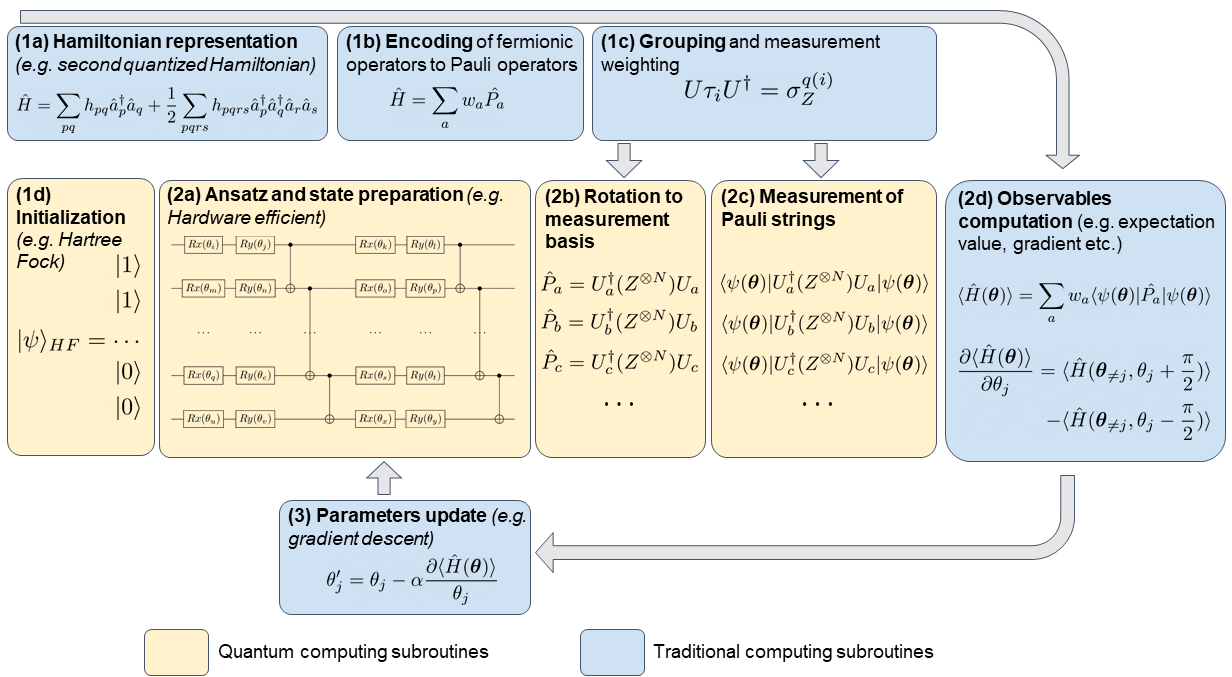
\includegraphics[width=\linewidth]{figs/VQE_pipeline.png}
    \caption{\textbf{The VQE Pipeline} - Formulas are illustrative and do not necessarily correspond to best practices. \textbf{(1) Pre-processing:}  \textbf{(a) Hamiltonian representation:} First pre-processing step of the VQE in which a set of basis functions is defined for the Hamiltonian to be expressed as a quantum observable of the electronic wave function (Sec. \ref{sec:Hamiltonian_representation}); \textbf{(b) Encoding:} Second pre-processing step of the VQE in which the Hamiltonian is encoded into a set of operators that can be measured on a Quantum Computer, using the qubit register wavefunction. To do this, fermionic operators in the Hamiltonian are mapped to spin operators using an encoding (Sec. \ref{sec:Encoding}); \textbf{(c) Grouping and measurement strategy:} Third step in the pre-processing, where operators defined in (b) are grouped in order to be measured simultaneously later on, usually requiring an add-on to the quantum circuit for each group in order to rotate the measurement basis in a basis in which all operators in the group are diagonalized. It is also the step in which we decide the measurement weighting strategy (Sec. \ref{sec:Grouping}); \textbf{(d) State initialization:} In this last pre-processing step, we decide how the state to which the ansatz is applied is initialized. In general, the Hartree-Fock wavefunction is used  \cite{Hartree1928, Slater1928, Gaunt1928, Hartree1935, Jensen2017}, but other options are briefly discussed in Sec. \ref{sec:ansatz_discussion} - \textbf{(2) The VQE loop:} \textbf{(a) Ansatz and trial state preparation:} The first step of the VQE loop is to apply the ansatz to the initialized qubit register, before the first iteration of the VQE all the parameters of the ansatz also need to be initialized (randomly or using a specific method, e.g. Ref. \cite{Grant2019, Patti2021}) (Sec. \ref{sec:Ansatz}); \textbf{(b) Basis rotation and measurement:} Once the trial wave function has been prepared, it must be rotated into the measurement basis of the operator of interest (quantum computers in general measure in the $Z$ basis), or a diagonal basis of a specific group of Pauli strings \textbf{(c) Observable computation:} The expectation value to be computed depend on the optimization strategy used, in any case however these are reconstituted by weighted summation on conventional hardware, or using a machine learning technique; \textbf{(d) Parameters update:} Based on the observables computed, and the optimization strategy, we can compute and apply updates to the ansatz parameters and begin a new iteration of the VQE (Sec. \ref{sec:Optimization}) - \textbf{(3) Post-processing, Error mitigation:} error mitigation is a layer of additional computation on measurement output (or directly on the quantum state prior to measurement) aimed at reducing the impact of quantum noise on the results (Sec. \ref{sec:error-mit})}
    \label{fig:VQE_pipeline}
\end{figure*}

It is worth briefly outlining the distinction between the VQE pipeline and that of other variational quantum algorithms (VQAs) \cite{cerezoVariationalQuantumAlgorithms2020}. The key distinguishing feature of VQE is that it is restricted to finding the eigenstate of a quantum observable, which is not necessarily the case of other VQAs (such as Quantum Approximation Optimization Algorithms \cite{Farhi2014} or the Variational Quantum Linear Solver \cite{BravoPrieto2019, Pellow-Jarman2021}). As such, the process of encoding the Hamiltonian is peculiar to VQE. Similarly, while all VQAs would benefit from efficient measurements, the nature of the observable used in VQE (often scaling polynomially in the system size) mean that efficient grouping and measurements strategies will likely have a far greater impact on the overall scaling of the method. 

A similar distinction can be drawn with the field of machine learning using Quantum Neural Networks (QNN) \cite{Kwak2021, Garcia2022}. While such methods can be considered as variational algorithms, the reverse is not necessarily true. Most VQAs, and the VQE, aim at finding the solution to a given problem from initial inputs. Machine learning on QNN aims at abstracting, and generalizing \cite{Abbas2021}, a pattern from already solved problems used as initial input. As such the algorithmic pipeline and challenges of both methods are largely different. In the case of QNN, one will be less concerned about the representation of the observable and poorly scaling measurement requirements. Instead, deciding on the process for encoding conventional data into a quantum state (often referred to as quantum feature map) \cite{Schuld2019, Huang2021_powerofdata} will be critical in determining potential for quantum advantage and is completely absent from the VQE pipeline. 

\subsection{Advantage argument, assumptions, and limitations of the VQE} \label{sec:VQE_advantage}

Quantum supremacy is achieved when algorithms running on quantum computers can produce results that surpass those generated on conventional computing resources in accuracy and/or resources required \cite{Preskill2013}. It was demonstrated on a tailored sampling task by several research teams \cite{Arute2019, Zhong2020, Wu2021, Madsen2022}, although the magnitude of the advantage has also been contested \cite{Pednault2021, Liu2021}. Quantum advantage is in general used interchangeably with quantum supremacy, however we propose to use quantum advantage to refer to an instance of quantum supremacy where the advantage has relevant, tangible applications. This concept can rely on theoretical scaling arguments or practical demonstrations. A precise definition of the resources required and of the accuracy metrics is required for any specific demonstration of quantum advantage, which needs to include all overheads and initialization requirements. Computing resources can be defined in many different ways, including overall absolute runtime, time scaling, memory requirements, or indeed `indirect' metrics such as the financial cost of the computation or energy consumption (for a discussion on the energy consumption of Quantum Computers, we recommend Ref. \cite{Jaschke2022}).

The VQE allows for the probabilistic measurement of observables over certain classes of parameterized approximate wavefunctions, which can neither be sampled from nor have their properties computed efficiently (e.g. in polynomial time) on conventional devices as the system size gets large. Of course, this implies that the Hamiltonians studied can be written as a polynomially growing sum of independent observables \cite{Peruzzo2014}, as is commonly found in a number of fields such as quantum chemistry, condensed matter physics, or nuclear physics. We provide a more detailed description of these specific classes of wavefunctions (the ansatz of the VQE) in Sec. \ref{sec:Ansatz}, while a comparison to alternative wavefunction classes, which can admit polynomial complexity on conventional computing resources, are described in Sec. \ref{sec:vqe_vs_conventional}. If these wavefunction forms, accessible via the VQE yet practically inaccessible via conventional means, admit sufficient accuracy in their approximation to the ground state, quantum advantage can be considered within this paradigm. The argument outlined above defines a necessary condition for the VQE to become a practically useful method for computing properties of quantum systems. It is clear from the literature, and outlined in Sec. \ref{sec:sota_vqe}, that under certain assumptions this condition is theoretically achievable \cite{Peruzzo2014, Barkoutsos2018, OMalley2016, Wecker2015, Lee2019, Wiersema2020}.

There are however many restrictions of quantum computing that this approach does not take into account, and we therefore propose two more stringent conditions. The first one is that VQE must demonstrate similar or higher accuracy than any conventional method, but with lower computational time-to-solution. This condition takes into account possible limitations due to hardware runtime, potentially resulting in a large pre-factor for VQE computations. In this review, the pre-factor refers to the multiplier applied to a scaling rule to obtain the actual run time of the method. If the VQE has better asymptotic scaling than conventional methods, but a large pre-factor, this means an advantage could only be achieved in the asymptotic regime of very large systems (with runtime possibly too large for VQE to be realistically usable). This would make it difficult to demonstrate quantum advantage for practical moderately sized systems. The second condition, which is also the most stringent form of quantum advantage for the VQE, is to achieve at least as good accuracy, and with faster compute time, for a system of sufficient complexity to accurately model a real problem of physical and chemical relevance. This involves demonstrations on systems, where the approximation error in defining the specific Hamiltonian for the original problem is of smaller magnitude than its solution using the VQE. This could be as simple as ensuring that basis sets are sufficiently saturated \cite{Jensen2017}, or that the complexity of the interactions with a wider system were sufficiently resolved. For instance, consider computing the energy of a series of protein-ligand complexes (for which methods extending VQE have already been proposed \cite{Malone2021, Kirsopp2021}): even if the VQE achieves better accuracy in lower computation time, it is not guaranteed that these accuracy gains lead to a practical advantage. For example, the accuracy gains may still be insufficient to predict the most appropriate ligand in a physical experiment due to the approximations in the treatment of the environment in the Hamiltonian. Some researchers have attempted to estimate the tipping point for quantum computing-based quantum chemistry to overtake conventional methods. As one example, Elfving {\it et al.} \cite{Elfving2020} estimate the size of basis set (and hence the number of qubits) that would be required for a tangible quantum advantage of quantum computing based methods to lie somewhere between $19$ and $34$ molecular orbitals (or twice as many spin orbitals and hence twice as many qubits).

Despite sound theoretical arguments for the polynomial scaling of VQE \cite{Peruzzo2014, mccleanTheoryVariationalHybrid2015}, a number of potential limitations have been identified as well, which could prevent the VQE from achieving quantum advantage:

\begin{itemize}
    \item The VQE could be limited by a large pre-factor linked to the cost of accurate observable sampling. Several studies have analyzed the overall cost of VQE and whether it can reach a tipping point, at which it becomes advantageous compared to conventional methods \cite{Wecker2015, Elfving2020, Gonthier2020}. They have so far all concluded that given certain assumptions and the current state of research surrounding VQE functionality, the algorithm cannot outperform conventional methods within a remit of applications considered tractable. The main bottleneck identified in these studies (based on noiseless estimates) is the substantial number of measurements that are required to estimate the expectation value of the Hamiltonian using VQE (for further details see Sec. \ref{sec:resource_estimates}). The field of research is fast-moving however, and much research has been devoted to efficient operator sampling (summarized in Sec. \ref{sec:Grouping}). Using the parallelization potential of VQE (see Sec. \ref{sec:parallelization}) could also be a solution to this measurement problem but would require a paradigm shift in the way quantum hardware is conceived.
    \item The VQE involves solving an optimization problem. As such, to understand the true cost of implementing VQE, one needs to assess the complexity of the optimization process. The true cost and scaling are dependent on the optimizer and on the optimization landscape of the specific problem studied. While some optimizers have been shown to converge in polynomial time for convex cost functions, the VQE is far from having such a favorable landscape \cite{Bittel2021, Anschuetz2022}. In fact, the VQE optimization is shown to be NP-hard \cite{Bittel2021}, which means that in the worst possible case, finding the optimal solution to the problem is intractable. Of course, this is to be expected as all optimization problems can suffer from the same issue \cite{Krentel1988}. The key open question is to know whether VQE can be optimized heuristically in a polynomial number of iterations and converge to an approximate yet accurate enough solution. 
    \item Even if one could show VQE would theoretically converge in a tractable number of iterations, this would assume that expectation values and gradients are computed exactly. This assumption is not valid in the context of quantum computation, and it has been shown that the number of measurements required to accurately measure gradients could scale exponentially in certain parameterizations of systems, due to the barren plateau problem  \cite{McClean2018} (discussed in detail in Sec. \ref{sec:barren_plateau}). A number of mitigating methods have been proposed, such as the identity block initialization \cite{Grant2019} or the use of a local encoding for the Hamiltonian \cite{Cerezo2021_BP, Uvarov2020}. Nevertheless, the extent to which barren plateaus can indeed be managed for VQE remains an open question. 
    \item Related to both of the above, the extent to which VQE is resilient to quantum noise is also an open question, but actively mitigating errors will likely be unavoidable for relevant use of NISQ algorithms. Although error mitigation methods have shown great success in improving the accuracy of VQE on the current generations of quantum computers (for instance \cite{Barron2020, Sagastizabal2019, Nam2020, Arute2020, Tilly2021, Benfenati2021}), it can significantly increase the resource requirements of the algorithm (see Sec. \ref{sec:error-mit}). It is unclear whether this increase in resources is an acceptable cost or likely to be a critical limitation in larger-scale application of the VQE. A recent paper~\cite{RyujiFundamentalLimits2021} is rather pessimistic on this point, showing that the increase in cost is exponential when the ansatz circuit grows deeper. Conversely, it was suggested in the early days of VQE that variational algorithms possess inherent noise resilience since the optimization can effectively adapt to the noise~\cite{mccleanTheoryVariationalHybrid2015}. This resilience has helped VQE to be more successful than other algorithms on the current generation of quantum devices, and has been numerically demonstrated in small qubit simulations \cite{Enrico2021EvaluatingNoiseResilience}. However, it remains unclear whether this resilience from noise can be retained in larger quantum experiments, where one is confronted with a more complex ansatz, with more noise coming from the difficulty of controlling large numbers of qubits with precision.
\end{itemize}

An important additional point to stress here is that while in theory the exact state could in principle be spanned by a number of qubits that scales linearly with system size, this exactness is in general forgone in VQE via the imposed parameterization. At this point, a strictly exact limit within a defined Hamiltonian is only expected to be recovered with an exponential number of variational parameters (and hence circuit depth) \cite{Evangelista2019}. Therefore, to achieve advantage, the classes of states accessible within the VQE framework must admit superior approximations to quantum many-body systems of interest compared to accessible conventional descriptions of quantum states, as well as their scaling with system size. The key question regarding the realm of current applicability of the VQE is therefore whether it can achieve higher accuracy on at least some representative systems, with some appropriate resource metric, compared to conventional computational chemistry methods.

\subsection{VQE and conventional computational chemistry} \label{sec:vqe_vs_conventional}

The first step in any application of VQE to {\em ab initio} electronic structure is to define the basis functions determining the resolution and representation of the system. A common (but not required) approach to this would be to use the molecular orbitals obtained from a prior mean-field Hartree-Fock (for a description of this method, see  Ref.~\cite{Jensen2017}) or density functional theory (DFT) calculation \cite{Hohenberg1964, Levy1979, Vignale1987, Kohn1965} (for comprehensive reviews of DFT, see Refs.~\cite{Parr1995, Bagayoko2014}). These orbitals are used to define the representation of the Hamiltonian (see Sec. \ref{sec:Hamiltonian_representation}), and thus compute the operator weights of the resulting Pauli strings. In this way, the VQE already relies on the techniques of conventional quantum chemistry for its use. Furthermore, in order to clarify the challenge for quantum advantage, as well as the expected scope and applicability of the VQE in the context of computational chemistry, we provide a very brief review of existing methods in this domain.

Although exceptions exist, it should be noted that most conventional approaches for high accuracy {\em ab initio} ground-state energetic properties of molecular systems rely on wavefunction approximations, in keeping with the wavefunction approximation inherent in the VQE approach \cite{Eriksen2020}.
Other quantum variables (such as densities, density matrices, or Green's functions) can be used, but are in general unable to reach state-of-the-art accuracy for ground state energies \cite{Williams2020}. As such, methods like DFT which is widely used in material sciences, and offers a competitive cost-accuracy trade-off for large systems are not direct competitors to VQE, due to the lack of systematic improvability of their results. Despite some quantum algorithms for electronic structure presenting algorithms with scalings competitive or even lower than DFT (for example, Ref.~\cite{Babbush2019}), the most likely competitors for short to medium term applications of VQE are accurate wavefunction approaches, which can scale as high polynomial or even exponential, but which still are able to access comparatively large system sizes.

\subsubsection{Full Configuration Interaction} \label{sec:full_configuration_interaction}

Full configuration interaction (FCI) provides the benchmark for exact representation of a quantum state for a given Hamiltonian and basis set \cite{Szabo1996,DavidSherrill1999}. This results in the approach being in most cases intractable, with practical limits for {\em ab initio} systems currently being 18 orbitals \cite{Vogiatzis2017}. However, its numerically exact treatment of the correlated physics ensures that it occupies a unique and important position in quantum chemistry and electronic structure. FCI builds the variationally optimal wavefunction as a linear superposition of all possible configurations of electrons within the available degrees of freedom.
Whilst the inclusion of all possible configurations ensures that the final result is invariant to the precise single-particle representation of the orbitals considered, it is common to perform FCI in a basis of Hartree-Fock molecular orbitals to improve the convergence rate. The Hartree-Fock method provides the variationally optimized single Slater determinant, as appropriate for closed-shell systems \cite{Jensen2017}, approximating the ground state wavefunction at the mean-field level. In this basis, the orbitals have individual single-particle energies associated with them, since they diagonalize the single-particle Fock matrix. The structure of the FCI wavefunction then takes the following form, where the configurations can be classed by the number of particle-hole excitations they create in the reference Hartree-Fock configuration, as

\begin{equation} \label{eq:CI_wf}
    \ket{\psi}_{\text{FCI}} = c_0 \ket{\psi}_{\text{HF}} + \sum_{ia} c_{ia} \hat{a}_a^{\dagger} \hat{a}_i \ket{\psi}_{\text{HF}} + \sum_{ijab} c_{ij, ab} \hat{a}_a^{\dagger} \hat{a}_b^{\dagger} \hat{a}_j \hat{a}_i \ket{\psi}_{\text{HF}} + \dots ,
\end{equation}
where the first sum represents `singly-excited' configurations where an occupied spin-orbital, denoted by the indices $i, j, \dots$ is depopulated, and a virtual spin-orbital, denoted by the indices $a, b, \dots$ is populated (here we use terminology corresponding to electronic structure theory, however these considerations are valid for any quantum system expressed in a finite basis). This (de)population is achieved while preserving antisymmetry of the overall wavefunction, via the use of the fermionic second quantized operators, $\hat{a}^{(\dagger)}$, with more details of these found in Sec.~\ref{sec:second_quantization}. These number preserving excitations from the reference Hartree-Fock determinant can be extended to double excitations (second sum) all the way up to $m$-fold excitations, where $m$ is the number of electrons. This then spans the full space of configurations, and due to the linear parameterization, ensures that the minimization of the Ritz functional (Eq.~\ref{eq:ritzfunc}) can be written as a diagonalization of the full Hamiltonian in this basis \cite{Ross1952,Foresman1996}. Exact excited states (within the defined basis and resulting Hamiltonian) can then also be computed as successively higher-lying eigenvalues of the Hamiltonian matrix in this basis. 

While the FCI represents the `ground truth' solution for the defined combination of Hamiltonian and basis set, the core aim of much of electronic structure is to truncate the complexity of this FCI solution (ideally to polynomial scaling with system size), while minimizing the loss in accuracy resulting from this truncation \cite{Szabo1996}. It is also advantageous to have the ability to systematically relax this truncation of the approximate ansatz, allowing for improvable results when the situation demands (for instance, see the methods described in Ref.~\cite{Eriksen2020}). To this end, a large number of approximate parameterizations of the FCI wavefunction have been explored, which differ in their accuracy, scaling, functional form, and method of optimization. Many of these approaches have enabled chemical accuracy and beyond compared the FCI result to be routinely reached in systems far larger than those accessible by FCI \cite{White1992,Sharma2012,Tubman2016, Booth2010,Thomas2015,Li2018}. The technical definition of chemical accuracy is specifically the accuracy required to compute accurate enthalpies (heats) of reactions, which numerically corresponds to a method achieving an output within $1.6$ milli-Hartree (mE$_{\rm H}$) \cite{Peterson2012} of experimental results. It is widely used as a benchmark for numerical methods, although it is worth noting that other chemical properties need higher accuracy (sometimes by 2 to 3 orders of magnitude for instance in the case of spectroscopic properties). It is in general considered extremely difficult (or impossible) to reach for large systems due to the approximations which are made when constructing the model. Oftentimes computational methods aim at a correct qualitative description of the chemical properties instead. We refer to chemical precision as the benchmark for the precision at which the model is solved, irrelevant of the uncertainties and approximation made when constructing the model (see Ref.~\cite{Elfving2020} for a thorough discussion of chemical accuracy vs. precision in the context of computational chemistry). 

The considerations described in devising an effective parameterization also largely echo the developments of ans\"atze for the VQE, although the functional forms of ans\"atze which admit efficient evaluation on quantum devices are different. In the next section, we explore a few of these parameterizations which are used on conventional devices, and how these considerations have influenced and transferred over to the choice of ansatz developed in the context of the VQE.

\subsubsection{Efficient approximate wavefunction parameterizations for conventional computation}

While the complexity of the exact FCI ansatz (Eq.~\ref{eq:CI_wf}) is clearly combinatorial with the number of degrees of freedom, many accurate and more compact wavefunction forms have been established. It results in more efficient approaches than FCI which can access larger system sizes, with only small tradeoffs in accuracy. As an illustration of the capabilities of state-of-the-art methods, a recent study presents a blind test comparison of nine different methods applied to benzene on an active space of $30$ electrons and $108$ molecular orbitals \cite{Eriksen2020}. The root mean square deviation between the results produced by these methods was only $1.3 \text{mE}_{\text{h}}$, demonstrating a consistent and reliable level of accuracy between these methods, expected to be close to FCI accuracy. A similar (albeit not blind) study was conducted in Ref.~\cite{Williams2020}, with applications to transition metal systems, again showing excellent agreement between the most accurate wavefunction methodologies in these systems.

To rationalize some of these parameterizations, an obvious first approximation to Eq.~(\ref{eq:CI_wf}) can be made via truncation in the total number of excitations from the reference configuration, allowing retention of the efficient linear form. The most common of these is the configuration interaction with singles and doubles ansatz (CISD), where only up to double excitations are retained \cite{Szabo1996}. More recent adaptive, selective or stochastic inclusion of desired configurations exploit the sparsity in the optimized amplitudes, and can extend the ansatz further in accuracy, resulting in methods such as Adaptive Sampling CI (ASCI) \cite{Tubman2016, Tubman2020, Hait2019, Levine2020}, Semistochastic Heat-Bath CI (SHCI) \cite{Petruzielo2012, Holmes2016, Holmes2016_2, Sharma2017, Smith2017, Holmes2017, Li2018}, or Full Configuration Interaction Quantum Monte Carlo \cite{Booth2010, Cleland2012, Anderson2020, Booth2011, Blunt2019}. However, these truncated linear approximations can suffer from size-intensive total energies, where the energy does not scale appropriately with respect to the number of electrons, ensuring that the energy error per particle becomes increasingly large as systems grow in size \cite{Szabo1996}. Nevertheless, they can result in excellent variational approximations to FCI for small systems. An alternative approach is to construct a multi-linear approximation to the FCI wavefunction, which results in the matrix product state functional form. This form can be efficiently optimized within the density matrix renormalization group (DMRG), and can also yield accurate and systematically improvable approximations to FCI both in the case of \textit{ab initio} molecular Hamiltonian and for lattice models \cite{White1992, White1993, White1999, Mitrushenkov2001, Legeza2003, Chan2002, Chan2011, Sharma2012, OlivaresAmaya2015, Wouters2014, Yanai2014, Knecht2016}. More broadly, the development of tensor network theory \cite{Biamonte2017, Ors2019} and the use of matrix product states has resulted in significant improvements of methods for the resolution of lattice models (for instance \cite{Schneider2021, Kaneko2022}). Finally, it is worth mentioning that a larger class of approximate wavefunction ansatz are able to be optimized within the framework of `Variational Monte Carlo'. In these approaches, an approximate ansatz is chosen whose probability amplitude can be efficiently sampled at arbitrary electron configurations, but where a closed-form polynomial expression for the energy of the state is not accessible \cite{TOULOUSE2016285,Needs2020,Pfau2020}. Within this criteria, the parameters of the ansatz can be optimized via Monte Carlo integration of the energy functional in a very general framework, albeit with the necessity of controlling for stochastic errors and care in optimization of the parameters. Many of these considerations transfer through to the VQE.

Largely to correct for the size inconsistency in linear ans\"atze, the popular coupled-cluster ansatz truncates and then exponentiates the form of Eq.~(\ref{eq:CI_wf}). This results in an appropriately sized consistent method, with an excellent accuracy vs. cost balance \cite{Eriksen2016_I, Eriksen2016_II, Ying2019}. The coupled-cluster with single, double and perturbative triple excitations retained in the ansatz (known as CCSD(T)) is often referred to as the `gold standard' of quantum chemistry where the correlations are not too strong \cite{Bartlett2007}, while other approximate coupled-cluster forms suitable for stronger correlation effects have also been developed (for recent examples, see Ref.~\cite{Wang2020_BCCC, Lyakh2011}). The coupled cluster is also the motivation of the use of the {\em unitary} coupled cluster ansatz of VQE \cite{Evangelista2019}, where a similar structure of exponentiated excitations based around a reference configuration is constructed (see Sec.\ref{sec:UCCA}), with modifications to ensure efficient use on a unitary set of quantum circuits. Similar considerations of dynamic inclusion of additional excitations is also possible with the ADAPT-VQE ansatz \cite{Grimsley2019} (Sec.~\ref{sec:adapt-vqe}). Furthermore, the Efficient Symmetry Preserving ansatz \cite{Gard2020} looks to ensure the ability to systematically improve its span of the FCI description of Eq.~(\ref{eq:CI_wf}) ensuring the preservation of symmetries inherent in its form. However, ensuring this systematic coverage of the FCI ansatz means that this form remains exponential in the system size in a number of realistic cases, meaning that true FCI may also be out of reach for the VQE.

An important consideration in the application of these approximate conventional parameterizations is that the size of the errors is different for different systems. Over time and use, an understanding has emerged from both theoretical and numerical analysis for the domain of applicability of these approaches and physical properties of the state which enable their accuracy, e.g. low-rank excitations (coupled cluster), locality (DMRG) or sparsity in the state (selected CI, FCIQMC). This understanding has promoted their effective use in appropriate circumstances, and stimulated further developments to improve their accuracy and scope. This analysis of the errors in different systems from VQE ansatz for quantum simulation, as well as the reasons underpinning or limiting their accuracy, is only starting to be performed, with more work necessary to fully classify and numerically investigate the approximations made in their form \cite{Evangelista2019, Grimsley2019_UCC_Review}.

Overall, these established wavefunction methods based on conventional computing (some of which are briefly described in this section) constitute the state of the art in high-accuracy quantum chemistry, at least for the ground state energetics. It should be stressed again that these approaches, as opposed to FCI, constitute the ultimate benchmark on which the success of VQE should be measured, as they represent approaches to systematically achieve chemical accuracy but with greater efficiency than exact FCI. This constitutes a demanding target for VQE to meet, with many decades of research in this area. Furthermore, continuing research for other parameterizations suitable for conventional devices, such as the rapidly emerging field of machine-learning inspired ans\"atze \cite{Carleo2017, Nomura2017, Choo2018, Glielmo2020, Luo2019, Pfau2020, Choo2020, Hermann2020}, will continue to push the boundaries of accuracy on conventional devices to challenge the criteria for VQE superiority.

\subsection{VQE and Quantum Phase Estimation} \label{sec:vqe_vs_qpe}
 
The Quantum Phase Estimation algorithm (QPE) \cite{Kitaev1995, Abrams1997, abramsQuantumAlgorithmProviding1998, Cleve1998, AspuruGuzik2005} provides a method to find a given eigenvalue of a Hamiltonian from an approximated eigenstate (ground or excited). QPE can compute an eigenvalue to a desired level of precision with a probability proportional to how close the approximated eigenstate is to the true eigenstate \cite{McClean2014}. It does so however using quantum circuits of depths that are far beyond what is achievable in the NISQ era of quantum computing \cite{reiherElucidatingReactionMechanisms2017}. As part of our discussion on the VQE we briefly outline QPE and how the two compare.    

\subsubsection{Overview of the quantum phase estimation}

A representation of the quantum circuit used to implement QPE is presented in Fig. \ref{fig:qpe_circuit}, and the process can be described as follows (adapting the descriptions in Refs. \cite{nielsenQuantumComputationQuantum2010, mcardleQuantumComputationalChemistry2018}):
\begin{itemize}
    \item The objective of QPE, like the objective of VQE, is essentially to compute an eigenvalue of a Hamiltonian. In the case of QPE however, the problem presented in Eq. (\ref{eq:vqe_cost_function}) is slightly reformulated. For a given Hamiltonian $\hat{H}$, and a given eigenstate $\ket{\lambda_j}$ (usually the ground state:  $\ket{\lambda_0}$), one tries to find a eigenvalue $E_j$ such that:
    \begin{equation} \label{eq:qpe_problem}
       e^{i\hat{H}} \ket{\lambda_j}= e^{ i E_j} \ket{\lambda_j}.
    \end{equation}
    The Hamiltonian is exponentiated to obtain a unitary operator, and without loss of generality we can write $e^{iE_j} = e^{2 \pi i\theta_j}$, with $\theta_j$ the `phase' QPE aims at discovering.
    \item The only inputs available however are the Hamiltonian, and an approximation of the ground state $\ket{\psi_0} \sim \ket{\lambda_0}$, which can be generally expressed in the eigenbasis of the Hamiltonian as 
    \begin{equation}
        \ket{\psi_0} = \sum_{j=0}^{2^{N_q}-1} \alpha_j \ket{\lambda_j},
    \end{equation}
    where $N_q$ is the number of qubits used to represent the electronic wavefunction of the Hamiltonian (which therefore has a total of $2^{N_q}$ eigenstates.
    \item A register of ancilla qubits is used to map the eigenvalue sought-after, in general to a binary number. The number of ancillas required therefore depends on the type of implementation and desired precision (more ancillas mean a longer binary string, and therefore a higher precision \cite{nielsenQuantumComputationQuantum2010}). This ancilla register is initialized as an equally weighted superposition of all possible state in the computational basis (all possible binary strings). If we have a total of $N_a$ ancilla qubits, there are $2^{N_a}$ such basis elements. Starting from a register in state $\ket{0}^{\otimes N_a}$, a Hadamard gate ($\Had$) is applied to each qubit (for readers requiring a brief introduction to key quantum computing concepts and operations, we recommend Sec. II.A of Ref.~\cite{mcardleQuantumComputationalChemistry2018}). We recall that $\Had\ket{0} = (\ket{0} + \ket{1})/\sqrt{2}$, and $\Had\ket{1} = (\ket{0} - \ket{1})/\sqrt{2}$. After these operations, the state of the ancilla register is
    \begin{equation}
        \ket{\psi_{\mathrm{anc}}} = \frac{1}{\left(\sqrt{2}\right)^{N_a}}\sum_{x=0}^{2^{N_a} - 1} \ket{\operatorname{bin}(x)},
    \end{equation} 
    where $x$ represents integers from 0 to $2^N_a - 1$ and $\operatorname{bin}(x)$ the binary representation of of $x$. When both the ground state approximation and the ancilla register are considered together we get the total state of the qubit register $\ket{\psi_{\mathrm{tot}}} = \ket{\psi_{\mathrm{anc}}}\otimes \ket{\psi_0}$ such that
    \begin{equation}
        \ket{\psi_{\mathrm{tot}}} = \left(\frac{1}{\left(\sqrt{2}\right)^{N_{a}}} \sum _{x=0}^{2^{N_{a}} -1}\ket{\operatorname{bin} (x)}\right) \otimes \left(\sum _{j=0}^{2^{N_{q}} -1} \alpha _{j}\ket{\lambda _{j}}\right) = \frac{1}{\left(\sqrt{2}\right)^{N_a}} \sum_{j=0}^{2^{N_q}-1} \sum_{x=0}^{2^{N_a} - 1} \alpha_j \ket{\operatorname{bin}(x)} \otimes \ket{\lambda_j}.
    \end{equation}    

    \item In the superposition state above, there is no clear relation between an ancilla state $\ket{\operatorname{bin}(x)}$ and the $j$-th eigenstate $\ket{\lambda_j}$. That is, if one were to measure the ancillas resulting in a binary number $\operatorname{bin}(x)$, no information could be gained about the state of the wavefunction register which encodes $\ket{\lambda_j}$, and therefore no information can be gained about the associated eigenvalues. In the following, we will apply unitary gates to this superposition state such that there is a clear one to one correspondence between a measured binary number $\operatorname{bin}(x)$ and the eigenvector $\ket{\lambda_j}$. Consider the following unitary
    \begin{equation} \label{eq:qpe_unitary}
        U^{(k)} = \left(e^{i\hat{H}}\right)^{2^k},
    \end{equation}
    with $k$ an arbitrary number for the time being. Following Eq. (\ref{eq:qpe_problem}), if this unitary is applied to eigenstate $\ket{\lambda_j}$, it effectively results in a phase $e^{(2\pi i\theta_j 2^k)}$. Now suppose that $k$ is the index of the ancilla qubits, i.e. $k \in [0, N_a - 1]$ and that, for each $k$, $U^{(k)}$ is applied to the ground state approximation only if the ancilla qubit of index $k$ is in state $\ket{1}$. This operation can be performed by mean of a controlled unitary operation, which applies a unitary operation subject to the value of a control qubit \cite{nielsenQuantumComputationQuantum2010}. For a superposition instance $\ket{\operatorname{bin}(x)}$ of the ancilla register, this means that the unitary $U$ is applied $x$ times in total to the ground state (consider for example the ancilla superposition $\ket{\operatorname{bin}(5)} = \ket{101}$, here qubits are indexed from right to left to correspond to binary strings. The unitary is applied for $k = 0$, and for $k = 2$, hence following Eq. (\ref{eq:qpe_unitary}) it is applied $5 = 1 \cdot 2^2 + 1 \cdot 2^0$ times). We obtain the state
    \begin{equation} \label{eq:qpe_post_CU}
        \ket{\psi_{\mathrm{tot}}} = \frac{1}{\left(\sqrt{2}\right)^{N_a}} \sum_{j=0}^{2^{N_q}-1} \sum_{x=0}^{2^{N_a} - 1} e^{2\pi i \theta_j x} \alpha_j \ket{\operatorname{bin}(x)} \ket{\lambda_j}.
    \end{equation}
    \item The next step reduces the number of superposition instances by applying an inverse quantum Fourier transform (QFT) to the ancilla register. QFT is a transformation from the computation basis to the Fourier basis, mapping a single computational basis element $\ket{\operatorname{bin}(y)}$ to a superposition of all computational basis elements each with different relative phase (due to the periodicity of the phase, each relative phase is a different point on the $2\pi$ period, with a total of $2^{N_a}$ different points)
    \begin{equation}
        \QFT\ket{\operatorname{bin}(y)} = \sum_{y=0}^{2^{N_a}-1} e^{2\pi i (xy / 2^{N_a})} \ket{\operatorname{bin}(x)}.
    \end{equation}
    If we set $y = 2^{N_a}\theta_i$, we can observe that applying the inverse QFT to the ancilla register in Eq.(\ref{eq:qpe_post_CU}) results in
    \begin{equation}
        (\QFT^{-1} \otimes I^{\otimes N_q}) \ket{\psi_{\mathrm{tot}}} = \sum_{j=0}^{2^{N_q} - 1} \alpha_j \ket{\operatorname{bin}(2^{N_a}\theta_j)} \ket{\lambda_j},
    \end{equation}
    where for simplicity we have assumed $2^{N_a}\theta_i \in \mathbb{N}$.
    \item Measuring the ancilla register in the $Z$ basis returns the binary string $\operatorname{bin}(2^{N_a}\theta_i)$ with probability $|\alpha_j|^2$, from which $\theta_i$, and $E_i$ can be recovered easily. The complete qubit register then collapses to the state $\ket{\operatorname{bin}(2^{N_a}\theta_i} \ket{\lambda_j}$.
\end{itemize}

\begin{figure}[ht]
\centerline{
        \Qcircuit @C=2.0em @R=1.5em {
          &      &\gate{\Had} & \qw & \qw & \qw & \hdots &  & \ctrl{4} &  \multigate{3}{\QFT^{-1}} &\meter  \\
            \lstick{\raisebox{1.2em}{ $\ket{0}^{\otimes N_q}$}} &\vdots&   &    &&  & \vdots &   & & & \vdots\\
          &      &\gate{\Had} & \qw & \ctrl{2} & \qw & \hdots &  & \qw &  \ghost{\QFT^{-1}} &\meter  \\
          &      &\gate{\Had} & \ctrl{1} & \qw  & \qw & \hdots &  & \qw &   \ghost{\QFT^{-1}} &\meter  \\
          \lstick{\raisebox{1.2em}{ $\ket{\psi_{\sim \lambda_0}}$}} &   & \qw & \gate{U^{(0))}} & \gate{U^{(1)}} & \qw & \hdots &  & \gate{U^{(N_q-1)}} & \qw & \qw
}
}\caption{Quantum circuit for Quantum Phase Estimation}  \label{fig:qpe_circuit}
\end{figure}

\subsubsection{Discussion and comparison}

Due to the ground state being measured directly in binary form in QPE, the number of ancilla qubits required is directly related to the precision $\epsilon$ targeted. Ancilla qubits provide one bit of information each, and as such, their number scales $\mathcal{O}(1/\log_2(\epsilon))$ in precision. The number of controlled unitaries is doubled for each ancilla qubit, and therefore scales $\mathcal{O}(1/\epsilon)$. These unitaries are effectively representing the action of the Hamiltonian on a state. The core component of QPE is therefore efficient Hamiltonian simulation (for an overview of relevant methods we recommend Ref.~\cite{Childs2018, Cao2019_QC}). Provided a non-restricted pool of qubits, Babbush \textit{et al.} \cite{Babbush2018} show that by engineering the correct Hamiltonian representation (namely, a plane wave basis in first quantization, see Sec. \ref{sec:Hamiltonian_representation}), one can achieve sub-linear scaling in the number of basis elements for Hamiltonian simulation.  

As mentioned above, QPE is only as likely to succeed as the fidelity of the input state to the unknown target eigenstate approaches one. In turn, this implies that using a randomized state as input is not an option as its expected fidelity to the target eigenstate approaches zero exponentially in the system size, resulting in QPE becoming exponentially costly with imperfect input state preparation \cite{McClean2014}. Numerous methods have indeed been proposed to prepare a good enough approximation of the target eigenstate in a tractable manner, often grounded in conventional quantum chemistry (for example\cite{tubman2018postponing, Sugisaki2018, Sugisaki2019, Motta2019, Murta2021}) or in adiabatic quantum computation (for example \cite{AspuruGuzik2005, Albash2018, Matsuura2020}). 

There have been a number of successful implementations of QPE on quantum devices \cite{Du2010, Lanyon2010, Li2011, Wang2015, OMalley2016, Paesani2017, Santagati2018}. These have only been on small systems, as large scale implementations require quantum resources which are not currently available. In particular, large scale controlled unitaries, required for QPE, cannot be reliably implemented on NISQ devices. This is also the case for the inverse QFT. Several numerical studies have been performed to assess the complete cost of implementing QPE on relevant systems, and estimate runtime on a fault tolerant quantum computer. The problem of nitrogen fixation has become a \textit{de facto} benchmark for this algorithm \cite{Beinert1997}. Reiher \textit{et al.} \cite{reiherElucidatingReactionMechanisms2017} estimates that the 54 electrons, 108 spin orbitals of $\mathrm{FeMo}$-co would require over $\mathcal{O}(10^{15})$ T gates, 200 millions qubits and would need to run for over a month to obtain quantitatively accurate results (assuming $100$ ns gate times and error threshold of $10^{-3}$). Berry \textit{et al.} rely on qubitization (a method which aims at transforming the evolution operator into a quantum walk) \cite{Low2019} to reduce the gate requirements to $\mathcal{O}(10^{11})$ Toffoli gates, despite an extended active space \cite{Li2019}. Lee \textit{et al.} \cite{Lee2021} further improve on these results and estimate they could perform this energy computation with four million physical qubits and under four days of runtime, with a similar $\mathcal{O}(10^{-3}$) error threshold. There have been many resource estimates performed for condensed matter models (for instance \cite{Babbush2018_Ham_Sim, Kivlichan2020}), with estimates as low as $\sim 500,000$ physical qubits running for a few hours to solve a $100$ site version of the Fermi-Hubbard model. Finally Elfving \textit{et al.} \cite{Elfving2020} estimate that with similar error rates, the chromium dimer ($\mathrm{Cr_2}$) with an active space of $52$ spin orbitals and $26$ electrons, would require $\mathcal{O}(10^{7})$ physical qubits running for about 110 hours. Research has progressed rapidly, and despite estimated runtimes and hardware requirements which remain daunting, offers a promising outlook for QPE, at least on targeted quantum chemistry tasks (examples of which are suggested in Ref.~\cite{Elfving2020}). 

The VQE trades off the depth and number of qubits required under QPE with a higher number of measurements and repetitions of the circuit, as well as the constraints of an approximate ansatz for the state. As presented in Ref.~\cite{Wang2019}, QPE requires $\mathcal{O}(1)$ repetitions with circuit depth scaling $\mathcal{O}(1/\epsilon)$ in precision $\epsilon$, VQE requires $\mathcal{O}(1/\epsilon^2)$ shots with circuit depth scaling $\mathcal{O}(1)$ in precision. While many other factors affect the overall time scaling of both methods, this point illustrates the asymptotic efficiency of QPE compared to VQE assuming access to fault tolerant quantum computers, but also the resource efficiency of VQE over QPE for NISQ-era devices. The frontier between NISQ and fault tolerant quantum computation is blurry, and as pointed out by Wang \textit{et al.} \cite{Wang2019} so is the frontier between VQE and QPE. They present an interpolation between the two algorithms, labeled Accelerated VQE (or $\alpha$-VQE), which uses smaller scale QPE calculations as sub-routines for the VQE. This method introduces a parameter $\alpha \in [0, 1]$ which allows tuning of the circuit depth $\mathcal{O}(1/\epsilon^{\alpha})$ and number of samples $\mathcal{O}(1/\epsilon^{2(1 - \alpha)})$ (one recovers the QPE scaling if $\alpha=1$, and the VQE scaling if $\alpha=0$). In general, rather than being mutually exclusive methods for solving an electronic structure problem, VQE and QPE are likely to provide the most benefit when combined as complementary approaches, offering algorithmic flexibility that can be adjusted depending on the progress of quantum hardware. 

\subsection{Our suggested best practices for VQE and their scaling assessment} \label{sec:sota_vqe}

In this section, we focus on combining compatible methods throughout the VQE pipeline, which offer the most promising scaling without compromising excessively on accuracy. The definition of a series of best practices for the VQE may suffer from many pitfalls since there remain many open research questions that affect the choice of optimal methods. It is also worth noting that it is likely that a method that is optimal for one system is not for another, and that this optimal compromise will change as quantum hardware improves.
With this in mind, we provide some suggestions for best practices on current devices for two broad families of systems. In particular, we can distinguish between lattice models \cite{Clark1997, nemoshkalenko1998computational,Marder2010, Continentino2021} and \textit{ab initio} molecular systems \cite{Parr1990, Friesner2005, Szabo1996, Jensen2017}. These two categories usually require different encodings, measurement strategies, and ans{\"{a}}tze. Table \ref{tab:sota_VQE} summarizes the most promising VQE methods that we have identified, together with their scaling. 
The key distinctive factor separating \textit{ab initio} molecular systems and lattice models is that the former makes no assumption on the range and type of interaction between the fermionic modes (beyond it being a two-body interaction), while the latter usually has a simplified and parameterized form which often only connects fermionic modes following a nearest-neighbor lattice structure and/or features a lower effective rank of interactions. 

As noted in the introduction, while the majority of the literature on VQE relates to electronic structure computation and lattice models, other applications have been proposed. Proposing best practices for these alternative applications is challenging as the research is sparse and therefore we avoid discussing these in this section. 

\begin{center}
% the width of columns are tuned
\begin{longtable}{p{2.5cm} p{2cm} p{5cm} p{5cm}}
\caption{Summary of state of the art methods identified for the VQE for both \textit{ab initio} molecular systems and lattice models. These methods and scalings are indicative only, as there remain a number of uncertainties with respect to their behavior on large scale systems and in noisy environments.} \label{tab:sota_VQE} \\
% -------------------------------
% first header
\hline\hline
\textbf{Task} & \textbf{\phantom{placeholder}} & \textbf{\textit{ab initio} Molecular systems} & \textbf{Lattice models}
\\ \hline 
\endfirsthead
% -------------------------------
% Shown as title on the next page 
% \bfseries make it bold. tablename creates: Table, thetable referes to the table's No.
\hline
\multicolumn{4}{c}{\bfseries \tablename\ \thetable{} -- continued from the previous page} 
\\ \hline
% -------------------------------
% replicate header on the second page
\hline \textbf{Task} & \textbf{\phantom{placeholder}} & \textbf{\textit{ab initio} Molecular system} & \textbf{Lattice models}
\\ \hline 
\endhead
% -------------------------------
% % Note: this foot note appears to be overlapping with
% % text surrounding it. Disable it atm:
\hline \multicolumn{4}{r}{{Continued on next page}} \\ \hline
\endfoot
\hline \hline
\endlastfoot
% -------------------------------------
% main table contents
\multirow{3}{=}{Hamiltonian construction \\(Sec. \ref{sec:Hamiltonian_representation})
} & Method & \textbf{Second quantization} & \textbf{Second quantization} 
\\
\phantom{} & Scaling & $\mathcal{O}(n^4)$ Hamiltonian terms and $N=\mathcal{O}(n)$ qubits, with $n$ number of basis functions & \textit{idem} \\
\phantom{} & Comments & First quantization could be advantageous on some systems, but further research is needed & \textit{idem} 
\\\hline % next row
\multirow{3}{=}{Fermion to spin encoding  \\(Sec. \ref{sec:Encoding})}
& Method & \textbf{Ternary tree Encoding} \cite{Jiang2020} & \textbf{Generalized Superfast Encoding} \cite{Setia2019} \\
\phantom{} & Scaling & Number of operators: $\mathcal{O}(N^4)$, Pauli weight $\mathcal{O}(\log_3(2N))$, & Qubit number: $N=\mathcal{O}(nd/2)$; for a regular lattice, number of operators scales $\mathcal{O}(ND)$, where $D$ is the lattice dimension; Pauli Weight: $\mathcal{O}(\log_2(d))$, with $d$ the fermionic-interaction graph maximum degree\\
\phantom{} & Comments & Low weight encodings could result in more resilience to barren plateau \cite{Cerezo2021_BP, Uvarov2020, Uvarov2020_frustrated}, and more compact ans\"atze, though there is at least some suggestions that it may increase impact of quantum noise \cite{Sawaya2016}  & \textit{idem}, the Compact encoding \cite{Derby2021, Derby2021_part2} results in a lower number of qubits for $D=2, 3$ but has not yet been generalized to higher dimensions. 
\\\hline % next row
\multirow{3}{=}{Grouping and measurement strategy \\ (Sec. \ref{sec:Grouping})}
& Method & \textbf{Decomposed interactions~} \cite{Huggins2021, Yen2021_Cartan} & \textbf{Qubit-wise commutation} \cite{mccleanTheoryVariationalHybrid2015, Kandala2017, Hempel2018, Rubin2018, Kokail2019, Izmaylov2019, Nam2020, Verteletskyi2020, Hamamura2020, Gokhale2019_long} \\
\phantom{} & Scaling & Operators to measure reduced to $\mathcal{O}(N)$; additional basis rotation circuit depth $\mathcal{O}(N/2)$ & Operators to measure reduced by a scalar, Additional basis rotation circuit depth $\mathcal{O}(1)$ \\
\phantom{} & Comments & Full rank optimization (in particular its extensions) \cite{Yen2021_Cartan} seem to achieve better overall measurement reduction for a given precision $\epsilon$ than the basis rotation method \cite{Huggins2021}, but cost scaling remains unclear. Classical shadows \cite{Huang2020} have been shown in at least one case \cite{OBrien2021} to outperform the scaling of decomposed interactions, though further numerical studies will be required to demonstrate dominance. & QWC grouping benefits from low Pauli weight encoding and comes at virtually no cost
\\\hline % next row
\multirow{3}{=}{Ansatz \\ (Sec. \ref{sec:Ansatz})} & Method & \textbf{k-UpCCGSD} \cite{Lee2019} & \textbf{Hamiltonian variational ansatz (HVA)~} \cite{Wecker2015, Wiersema2020}\\
\phantom{} & Scaling & Circuit depth of $\mathcal{O}(kN)$, number of parameters $\mathcal{O}(kN^2)$ & Circuit depth and number of parameters: $\mathcal{O}(k\tilde{C})$, with $\tilde{C}$ the number of commutative groups in the Hamiltonian (at most $\mathcal{O}(ND)$ for a regular lattice)\\
\phantom{} & Comments & Promising scaling, and good accuracy \cite{Lee2019, Grimsley2019_UCC_Review} but uncertainty remains for applications on large highly correlated systems. Uncertainty around $k$, the number of repetitions required. Adaptive ans\"atze \cite{Grimsley2019, Yordanov2020_IQEB, Tang2021} may perform better, but their scaling requires more investigation. & HVA has shown resilience to barren plateau and efficacy on lattice models \cite{Wiersema2020}. $k$ is the number of repetition of the anstaz required to reach the desired accuracy.
\\\hline % next row
\multirow{3}{=}{Optimizer \\ (Sec. \ref{sec:Optimization})} & Method & \textbf{Rotosolve} \cite{Vidal2018,nakanishi_sequential_2020,ostaszewskiStructureOptimizationParameterized2021} or \textbf{Fraxis} \cite{Watanabe2021WatanabeOptimizingSelection, Wada2021SimulatingCircuits} & \textbf{Rotosolve} \cite{Vidal2018,nakanishi_sequential_2020,ostaszewskiStructureOptimizationParameterized2021} or \textbf{Fraxis} \cite{Watanabe2021WatanabeOptimizingSelection, Wada2021SimulatingCircuits}\\
\phantom{} & Scaling & Requires sampling three values for each parameter at each step & \textit{idem} \\
\phantom{} & Comments & Some indication of faster convergence \cite{ostaszewskiStructureOptimizationParameterized2021}, but does not allow for full potential for parallelization of VQE, and requires more values to sample than most optimizers & \textit{idem}
\\\hline % next row
\multirow{3}{=}{Error mitigation strategy \\ (Sec. \ref{sec:error-mit})}
& Method & \textbf{Symmetry verification} \cite{mcardleErrorMitigatedDigitalQuantum2019,bonet-monroigLowcostErrorMitigation2018} and \textbf{extrapolation based methods} \cite{temmeErrorMitigationShortDepth2017,liEfficientVariationalQuantum2017} & \textit{idem} \\
\phantom{} & Scaling & Exponential with respect to the circuit depth & \textit{idem} \\
\phantom{} & Comments & 
%There is not a clear best error mitigation strategy, although extrapolation and symmetry based methods are promising due to their extensive applications and simplicity.
The recommendation reflects the \textit{de facto} method of choice for experiments. A fair comparison of the performance and cost between different error mitigation methods requires further research.
& \textit{idem}
\\ \hline\hline
\end{longtable}
\end{center}

\subsubsection{Best practices for \textit{ab initio} electronic structure of molecular systems}

\paragraph{Hamiltonian construction:} In the case of an \textit{ab initio} molecular system, the Hamiltonian representing its electronic energy landscape is initially defined by a series of atoms and the spatial coordinates of their nuclei (see Sec. \ref{sec:Hamiltonian_representation}). The first choice to make is the basis in which the Hamiltonian is expressed. This directly impacts the number of qubits required for the implementation of VQE, which is proportional to the number of basis functions. Since the number of qubits is a limited resource in NISQ, we recommend using a molecular orbital basis, as it is in general more compact for a given target accuracy (compared to, for example, atomic or plane wave bases). Once a basis is decided upon, we must choose whether the Hamiltonian is prepared in first quantization (antisymmetry maintained by the wavefunction) or second quantization (antisymmetry maintained by the operators, see Sec. \ref{sec:Hamiltonian_representation}). The number of qubits in first quantization scales as $\mathcal{O}(m\log_2(n))$ \cite{Abrams1997, Berry2018}, with $m$ the number of electrons and $n$ the number of basis functions, against $\mathcal{O}(n)$ in second quantization \cite{Jordan1928}. The former also requires additional depth to enforce the antisymmetry of the wavefunction. There has not been, to the best of our knowledge, a rigorous study of the efficiency of using first quantization in VQE. While the scaling for first quantization could be advantageous in systems with few electrons and large basis sets (e.g. if a plane wave basis is used \cite{Babbush2018}), second quantization is generally preferred. 

\paragraph{Encoding:} The next decision to take is that of the mapping used to transform the fermionic, second quantized Hamiltonian into a weighted sum of Pauli operators (see Sec. \ref{sec:Encoding}). The most relevant encodings for \textit{ab initio} molecular system include Jordan-Wigner \cite{Jordan1928}, the Parity \cite{Seeley2012}, Bravyi-Kitaev \cite{Bravyi2002, Seeley2012, Tranter2015}, and ternary tree mappings \cite{Jiang2020} (all are explained in detail in Sec. \ref{sec:gen_encoding}). Out of these, the most promising encoding is the ternary tree mapping \cite{Jiang2020}, since asymptotically it has the lowest Pauli weight (maximum number of non-identity Pauli operators in the string), resulting in lower circuit depth and possibly higher resilience to the barren plateau problem \cite{Cerezo2021_BP, Uvarov2020}. It is however still unclear whether this lower circuit depth does indeed result in more noise resilience, as pointed out in Ref. \cite{Sawaya2016}. We also recommend that the resulting qubit Hamiltonian is further reduced using tapering off methods based on symmetries \cite{bravyi_tapering_2017, Setia2020, Kirby2021_CSVQE} (see Sec. \ref{sec:tappering_qubits}).

\paragraph{Measurement strategy:} The large number of measurements required to sample the numerous terms in the Hamiltonian is often cited as the most detrimental bottleneck of VQE \cite{Wecker2015, Elfving2020, Gonthier2020}. Deciding on an efficient strategy for grouping and measuring Hamiltonian terms can go a long way in reducing this bottleneck. The decomposed interactions methods \cite{Huggins2021, Yen2021_Cartan} provide on balance the most promising means to jointly measure the Hamiltonian. They allow measuring an entire molecular Hamiltonian with $\mathcal{O}(N)$ groups (for more details about this method, see Sec. \ref{sec:DecomposedInteractions}) and require additional circuit depth of $\mathcal{O}(N)$ to perform the necessary basis rotation, which is usually acceptable since this scaling is equivalent or better than for most ans{\"{a}}tze. While it was shown that methods using grouping based on general commutativity of Pauli strings (e.g. \cite{Gokhale2019_short, Hamamura2020}) require fewer shots to achieve a given accuracy \cite{Yen2021_Cartan} in some numerical studies (in particular when using the Sorted Insertion heuristic \cite{Crawford2021}), this reduction will likely not be worth the additional circuit depth scaling $\mathcal{O}(N^2)$ \cite{Gokhale2019_long} required to perform the joint measurements. It is also worth noting that among the decomposed interactions methods, the Variance-estimate Greedy Full Rank Optimization \cite{Yen2021_Cartan} appears to perform best, although it requires minimization search of decomposition parameters. While this cost could be tractable there has been, to the best of our knowledge, no thorough research on how it would scale on large systems. For this reason, the Basis Rotation Group methods \cite{Huggins2021}, which have a predictable cost, is a more cautious choice currently. For additional efficiencies and variance reduction, one can distribute shots according to the weights of each group in the Hamiltonian \cite{Wecker2015, Rubin2018,Arrasmith2020}. It is worth noting however that the $\mathcal{O}(N)$ scaling in number of groups is not an ideal proxy for the scaling in number of measurements required to achieve a given precision on observable estimation. This is due to possible covariances arising from the joint measurement of different operators \cite{mccleanTheoryVariationalHybrid2015}. Classical shadows \cite{Huang2020} is also a promising method for reducing measurement count in VQE and has been shown in one study to have a better asymptotic scaling than decomposed interactions \cite{OBrien2021}. Further numerical studies will be required to establish the true performance of classical shadows compared to grouping methods.  

\paragraph{Ansatz:} We now have to decide on an ansatz to model the electronic wavefunction on the qubit register. Deciding on an ansatz remains challenging because it is often unclear which is expressive and efficient enough to allow for a good approximation of the ground state. The ansatz with the best scaling, and some evidence for appropriate accuracy for the ground state representation \cite{Grimsley2019_UCC_Review}, is the Unitary paired Generalized Coupled Cluster Singles and Doubles (UpCCGSD) ansatz \cite{Lee2019} (see Sec. \ref{sec:Ansatz} for a detailed description). This ansatz scales linearly with the number of qubit $\mathcal{O}(kN)$, but may require to be repeated $k$ times to reach the desired accuracy. The scaling of required repetition of the ansatz $k$ has been partially studied \cite{Lee2019} but remains uncertain for large systems. This ansatz also has the advantage of only needing a fairly low number of parameters ($\mathcal{O}(kN^2)$). Adaptive ans\"atze (such as ADAPT-VQE \cite{Grimsley2019}, iterative Qubit Coupled Cluster \cite{Ryabinkin2020} and Cluster VQE \cite{Zhang2020}) are also promising, as they may provide resilience against barren plateaus. Their main drawback is that these adaptative methods come at the cost of selecting an operator to grow the ansatz (or Hamiltonian) and the need to fully re-optimize the ansatz at each iteration. Numerical studies have suggested that additional measurements may be required compared to fixed structure ans\"atze \cite{Claudino2020}, although further research is required to provide an exhaustive costs and benefits analysis.

\paragraph{Optimizer:} It is challenging to systematically compare different optimizers since no thorough large scale studies of their convergence rate have been conducted. For the time being, the Rotosolve optimizer \cite{Vidal2018,nakanishi_sequential_2020,ostaszewskiStructureOptimizationParameterized2021} (see Sec. \ref{sec:analytical_opt}) has been shown to converge significantly faster than several gradient based optimizers \cite{ostaszewskiStructureOptimizationParameterized2021}. It offers the advantage of not relying on any meta-parameters (such as a learning rate), which makes it a very easy optimizer to implement. However, Rotosolve presents two significant caveats: firstly, each iteration requires sampling three different values instead of two for most gradient based methods (one can avoid this overhead by finding one of the values from the optimization of the previous parameter, but this could result in correlated noise); secondly, parameters must be updated sequentially, thereby restricting the scope for parallelization of the VQE. The Fraxis method \cite{Watanabe2021WatanabeOptimizingSelection, Wada2021SimulatingCircuits} works in a similar manner and has been shown in some numerical studies to perform at least as good as Rotosolve or even outperform it. For the time being, given there are currently no optimizers that have been shown to have superior convergence rates, and given we do not expect that there will be a sufficient number of quantum computers to fully exploit the parallelization potential of the VQE in the NISQ era (see Sec. \ref{sec:parallelization}), we propose the Rotosolve / Fraxis optimizers over other alternatives (although it is worth noting that the Quantum Natural Gradient \cite{koczor_quantum_2020} has been shown to perform well and to benefit from resilience to barren plateaus \cite{stokes_quantum_2020,McArdle2019}, albeit at a significant cost \cite{koczor_quantum_2020}). 

\paragraph{Scaling:} Based on the discussion above, we can now construct a scaling estimate for a single iteration of the state-of-the-art VQE for \textit{ab initio} molecular systems. The overall scaling is expressed in terms of the number of quantum gate time steps that must be performed (i.e. several gates applied on disjoint sets of qubits can be implemented within the same time step). The computation of the expectation value of a single operator at a precision $\epsilon$ requires $\mathcal{O}(1/\epsilon^2)$ repetitions of the ansatz. In principle, $\epsilon$ should aim for chemical precision, generally accepted as 1.6 mE$_{\rm H} \approx 10^{-3} $E$_{\rm H}$. However, it is worth noting that, in practice gradients may become lower than chemical precision (due to the barren plateau problem for instance, described in Sec. \ref{sec:barren_plateau}). In this situation, estimating gradients may require a more precise $\epsilon$ and more measurements, but it also means that optimization may rapidly become impossible.  
If the k-UpCCGSD ansatz is chosen, this scales as $\mathcal{O}(kN)$, while choosing to use the decomposed interactions of Sec.~\ref{sec:DecomposedInteractions} requires $\mathcal{O}(N)$ different operators to be measured (and therefore a gate depth of $\mathcal{O}(N)$ for rotation to the joint measurement basis) resulting in a total scaling for a single estimation of the entire Hamiltonian of $\mathcal{O}(kN^2/\epsilon^2)$. 
%Up until this point, all of the computation mentioned can be parallelized, i.e. this scaling can be reduced by an equivalent number of quantum computer cores, or threads (for a discussion on parallelization in the context of VQE, see Sec. \ref{sec:measurements_strategies}).

There are $\mathcal{O}(kN^2)$ parameters in the k-UpCCGSD ansatz, hence this represents the cost scaling of updating each parameter using the Rotosolve optimizer. As this optimizer is not parallelizable, one may prefer to use a different method if sufficient sets of qubits are available. Overall, this gives us a total scaling for one iteration of the VQE of $\mathcal{O}(k^2N^4/\epsilon^2)$ without parallelization, and $\mathcal{O}(kN)$ with full parallelization (the circuit depth). This perfect parallelization would require $\mathcal{O}(kN^3/\epsilon^2)$ sets of $\mathcal{O}(N)$ qubits. Note that while qubits within one set need to be entangled for the course of a single measurement, there is no requirement for entanglement between qubits of different sets of parallel quantum compute nodes. The sets of qubits can therefore be either all within on one quantum computer, or else also distributed across different separated quantum computers (see Sec. \ref{sec:parallelization}). It should be noted that the precision $\epsilon$ is generally required to achieve chemical precision. However, if a barren plateau occurs, $\epsilon$ may need to be reduced by orders of magnitude to compute gradients accurately enough to achieve a satisfactory optimization.

So far we have only considered the scaling of one iteration. It is still an open research question how the number of iterations required to achieve convergence scales with system size for the VQE. This depends on numerous factors, including the ansatz, the optimizer used, and the system studied. One important point to note is that convergence tends to be rapid at the beginning of the optimization process, with large gradients that require only a low number of shots to be computed accurately enough to progress. It becomes more challenging close to the optimum, where gradients are smaller, requiring a larger number of shots to continue the optimization. As such the last few iterations of the VQE are likely orders of magnitude more expensive than the rest of the optimization, if the algorithm is implemented efficiently.  

There are other overheads that may be worth consideration in the initial setup of the system Hamiltonian. The computation of the Hamiltonian matrix elements generally has a polynomial scaling, while naive implementations of Hartree-Fock scale $\mathcal{O}(n^4)$ \cite{Koppl2016}, with $n$ the number of basis functions, and it can be reasonably assumed that $n=N$ for \textit{ab initio} molecular systems. Similarly, applying a decomposed interactions method to diagonalize operators and reduce measurements requires rewriting the Hamiltonian in a different basis \cite{Huggins2021, Yen2021_Cartan}. However, these costs only occur once at the beginning of the VQE process, and are unlikely to be a bottleneck. Despite possibly higher scaling than that of a VQE iteration, they are likely to have a significantly lower pre-factor (as implemented on conventional hardware), and as such are not likely to constrain  the application of the algorithm except far in the asymptotic realm. However, less investigated is that these joint measurement bases may result in covariance between measurements of different Hamiltonian terms, thereby requiring additional measurements \cite{mccleanTheoryVariationalHybrid2015, Crawford2021, Huggins2021, Yen2021_Cartan} which could significantly affect overall cost for the VQE.

\subsubsection{Best practices for lattice models}

Our suggestions for lattice models differ from their {\em ab initio} counterparts. Lattice models for the most part only include terms in the Hamiltonian between nearest-neighbors on their respective lattice, with interactions between more distant sites significantly truncated in range. 
%Significant efficiencies can be gained by recognizing the fact that the methods developed for \textit{ab initio} molecular systems do not neglect these distant interactions. 
In particular, this limited degree of connectivity of lattice models provides the option to construct mappings with much lower Pauli weight, enabling more compact ans{\"{a}}tze to be efficient, though this can come at the cost of additional qubits.

\paragraph{Hamiltonian construction:} In the case of a lattice model, the Hamiltonian is given as a small number of empirical parameters, requiring no prior computation of matrix elements. These models are generally most naturally and efficiently expressed in terms of fermionic operators in the site representation, where the locality of the interaction can be exploited to reduce the number of measurements. %Similar to \textit{ab initio} molecular systems, first quantization could require significantly more qubits, but could still offer an advantage for some systems (e.g. systems that are represented with a large number of plane wave basis functions). Until demonstrated otherwise, second quantization is the preferred option. 

\paragraph{Encoding:} There is significant literature on the fermion-to-spin mapping for lattice models (see Sec. \ref{sec:lattice_encoding} for further details). These mappings are in general designed to minimize the required Pauli weight of the operators for a given lattice structure. The most important property of a lattice is the maximum degree of connectivity (coordination) of the sites, denoted $d$. For instance, a square lattice has $d=4$, and an equivalent hypercubic lattice of dimension $D$ has $d=2D$. 
If one is limited by the number of qubits available, the most appropriate mapping for a lattice is an adaptation of the Bravyi-Kitaev mapping (based on Fenwick trees) \cite{Havlek2017}, and which has a Pauli weight scaling as $\mathcal{O}(\log(v))$, where $v$ is the minimum number of sites in any one dimension for a $D=2$ lattice. It has the advantage of reducing the Pauli weight of the operators produced, compared to a naive implementation of Bravyi-Kitaev on a lattice, while maintaining the number of qubits required equal to the number of sites, $n$. If however the number of qubits is not a hard constraint, the Generalized Superfast Encoding method \cite{Setia2019} provides a lower Pauli weight scaling of $\mathcal{O}(\log_2(d))$ at the cost of requiring an increased number of qubits for each site, with an overall scaling of $\mathcal{O}(nd/2)$ qubits. The Compact encoding \cite{Derby2021, Derby2021_part2} requires a lower number of qubits ($\sim 1.5n$), but has not yet been generalized for regular lattices of more than three dimensions.  
Beyond their relationship to the resilience to barren plateaus in the optimization \cite{Cerezo2021_BP, Uvarov2020, Uvarov2020_frustrated}, the relevance of the Pauli weight in the context of VQE is also in how it affects the choice of ansatz, and in particular whether the ansatz is initially expressed in terms of fermionic operators. If the chosen ansatz is not dependent on fermionic terms, then Bravyi-Kiteav or Jordan-Wigner mappings are preferred. Furthermore, the number of qubits required to represent the Hamiltonian can be reduced using the tapering off methods based on symmetries as described in Sec.~\ref{sec:tappering_qubits} \cite{bravyi_tapering_2017, Setia2020}. 

\paragraph{Grouping and measurement strategy: } 
The number of operators in lattice models scales, in general, with the number of edges of the lattice graph, $E$. For example, for a hypercubic lattice of dimension $D$, the number of edges, and therefore, the number of operators will scale $\mathcal{O}(nD)$ (though it is worth noting that the pre-factor to this scaling may change significantly depending on the encoding used), as detailed in Sec. \ref{sec:lattice_encoding}. Because it is in general possible to reach low Pauli-weight encodings for lattice models (see Sec. \ref{sec:lattice_encoding}), qubit-wise commutativity (QWC) grouping \cite{mccleanTheoryVariationalHybrid2015, Kandala2017, Hempel2018, Rubin2018, Kokail2019, Izmaylov2019, Nam2020, Verteletskyi2020, Hamamura2020, Gokhale2019_long} could possibly offer significant potential for reductions in the number of terms. It is also worth considering the fact that ans\"atze for lattice models tend to be shallower, and as such, the cost of basis rotations in methods based on general commutativity of Pauli operators could be too significant to justify its use. As such we would therefore recommend QWC grouping until further research is conducted.

\paragraph{Ansatz:} Direct application of ans{\"{a}}tze suited for \textit{ab initio} molecular systems (such as Unitary Coupled Cluster, UCCSD and its extensions) have been shown to work in practice using generalized encodings such as Jordan-Wigner (see for instance, Ref.~\cite{Sokolov2020}). However, we note that the underlying physics motivating the ansatz is not ideally suited to strongly correlated lattice models, requiring care to ensure that they are efficient ansatz for these systems \cite{Evangelista2019}. Since these ans\"atze are formulated in a basis of Hartree-Fock or other mean-field orbitals, they do not allow using some of the low-weight encodings easily and do not enable exploitation of the low degree of connectivity of the model. Instead, one ansatz that has been shown to be very suitable for correlated lattice problems is the Hamiltonian variational ansatz (HVA) \cite{Wecker2015, Wiersema2020} (see Sec. \ref{sec:hva}). The ansatz leverages the more compact structure of the lattice model Hamiltonian and is built using fermionic operators, thereby making the most of low Pauli weight lattice encodings \cite{Setia2018, Setia2019, Derby2021, Derby2021_part2}. HVA was also shown in \cite{Wiersema2020} to be particularly resilient to the appearance of barren plateaus in the optimization problem. The ansatz has a depth and number of parameters scaling with the number of commutative Pauli groups in the Hamiltonian (though it may need to be repeated several times to account for lower expressibility compared to UCCSD). For a regular lattice, this can result in an overall scaling that is lower than $\mathcal{O}(nD)$. Extensions of HVA could also be considered for specific systems. For instance, Fourier Transform-HVA \cite{Babbush2018} could be very efficient on certain models (in particular jellium in Ref.~ \cite{Babbush2018}, which is a continuous model, but with the Hamiltonian defined by a single parameter). Symmetry breaking HVAs \cite{Vogt2020,Choquette2021} are also a promising avenue, and though numerical tests from Ref.~\cite{Choquette2021} show excellent fidelities of the state produced, results in Ref.~\cite{Vogt2020} show some instabilities of the ansatz. Overall, until further research is conducted, we consider that HVA is safest and most general option for lattice models. Finally, we have neglected consideration of adaptive ans{\"{a}}tze, as it is difficult to make a scaling argument for their efficiency in this domain, where the ability to justify the inclusion of some terms over others in the ansatz is likely to be diminished.

\paragraph{Optimizer: } Similar to our proposal for \textit{ab initio} molecular systems presented earlier, we find that Rotosolve \cite{Vidal2018, nakanishi_sequential_2020,ostaszewskiStructureOptimizationParameterized2021} and Fraxis \cite{Watanabe2021WatanabeOptimizingSelection, Wada2021SimulatingCircuits} currently have the best supporting evidence among the optimizers available.

\paragraph{Scaling:} Based on the above, we can make an argument for the scaling of VQE as implemented for lattice models. The number of shots required to achieve a precision of $\epsilon$ when computing an expectation value scales $\mathcal{O}(1/\epsilon^2)$, with $\epsilon$ the target precision. For lattice models however, the target is usually not chemical accuracy and instead depends on the aim of the calculation. Generally, the aim is to resolve some correlated features of the electronic structure (e.g. predicting the parameter regimes for different phases, or response properties Ref.~\cite{Fan1970, Marro1999, Stanislavchuk2015, Choi2019}). The HVA ansatz has a scaling capped by the number of terms in the lattice model Hamiltonian and the number of repetitions of the ansatz $k$, hence $\mathcal{O}(knD)$. However, there may be a few caveats to this. Since some encodings require additional qubits to reduce the Pauli weight, they would increase the depth and the number of terms in the ansatz, while at the same time reducing the depth per term of the ansatz due to the reduced Pauli weight. Overall these two effects are likely to only affect the pre-factor of the VQE, noting that we consider this an area of open research. Therefore, we maintain the previous scaling and estimate that a single energy evaluation would scale $\mathcal{O}(k(nD/\epsilon)^2)$. 

For a regular hypercubic lattice with only at most nearest-neighbor terms in the Hamiltonian, there are $\mathcal{O}(knD)$ parameters in the HVA, bringing the total scaling of computing gradients for a lattice model VQE to $\mathcal{O}((knD)^3/(\epsilon)^2)$. As noted previously, if the full parallelization potential is exploited, this would give a scaling of $\mathcal{O}(knD)$ for one iteration of the VQE. Discussions regarding the number of iteration are identical to the considerations raised in the previous section. It is worth noting that there has been so far no evidence that qubit-wise commutativity grouping can reduce the overall scaling of the number of operators to measure, and therefore we have not included it in this scaling analysis. Similarly, while the depth of HVA scales with the number of commutative groups in the Hamiltonian, we have not yet found an argument on whether this would reduce scaling below that of the number of terms $\mathcal{O}(nD)$.

\subsection{Resource estimate for VQE} \label{sec:resource_estimates}

\subsubsection{Cost and runtime estimates for VQE}

There have been several studies estimating the resources required to perform VQE on a system that is too large to be accurately treated using conventional methods. Wecker et al. \cite{Wecker2015} develops the Hamiltonian Variational Ansatz (HVA), and presents a numerical study of the accuracy of certain ans{\"{a}}tze (the HVA and various UCC based ans{\"{a}}tze) and the number of repetitions required. They also possibly unveiled the existence of the barren plateau problem ahead of it being characterized in Ref. \cite{McClean2018}, by numerically showing that more expressive forms of UCC cannot reach the same accuracy as less expressive forms on larger systems. They estimate that the total number of samples required to compute the ground state energy of $\mathrm{Fe_2S_2}$ to chemical precision (using the STO-3G basis with $n=112$ spin orbitals) is of the order $\mathcal{O}(10^{19})$, which is far beyond what could be considered tractable. Of course, conventional methods aiming at resolving exactly, and directly, the ground state of a $n=112$ spin orbitals Hamiltonian would also be intractable (this would equate to finding the lowest eigenvalue of a $2^{112}$ matrix). However this does not exclude the possibility that more refined conventional methods, accepting some approximation, could an acceptable level of accuracy on $\mathrm{Fe_2S_2}$ (as an example, please see Ref. \cite{Li2013}). The literature has progressed significantly since this 2015 study, and there are now more efficient ans\"atze (see Sec. \ref{sec:Ansatz}) and grouping methods (see Sec. \ref{sec:Grouping}) that may change this conclusion. 

K\"uhn \textit{et al.} \cite{Kuhn2019} numerically assess the number of qubits and circuit depths required for UCC based ans{\"{a}}tze. They show that to model a medium-sized organic molecule such as naphthalene ($\mathrm{C_{10}H_8}$, with $68$ electrons) would roughly require about $800$ to $1500$ qubits, and a number of two-qubit gates of about $\mathcal{O}(10^8)$ using UCCSD. This latter number may be significantly lowered if the k-UpCCGSD ansatz is used (assuming it can achieve the desired accuracy). They also claim that the run time for a VQE implementation would be impractical, even using full parallelization potential, without unfortunately providing more details about how this conclusion is reached. 

Gonthier {\it et al.} \cite{Gonthier2020} provide what probably constitutes the most comprehensive study of the VQE resource requirements to date by estimating the cost of combustion energy computation for nine organic molecules (including methane, ethanol, and propane). They provide a detailed estimate of the runtime for one energy estimation ranging from $1.9$ days for methane ($\mathrm{CH_4}$), which requires $104$ qubits for accurate treatment, to $71$ days for ethanol ($\mathrm{C_2H_6O}$), which requires 260 qubits (this estimate uses a frozen natural orbital basis, with 13 functions, i.e. 13 qubits for each electron). The analysis is rather exhaustive since it takes into consideration the joint measurements of Hamiltonian terms (see Sec. \ref{sec:Grouping}), and different optimization methods (see Sec. \ref{sec:measurements_strategies}). 

It is worth noting that the studies mentioned above do not take into account the three obstacles we listed at the beginning of this section (namely, the complexity of the optimization, the barren plateau problem, and the impact of quantum noise). At the same time, Refs.~\cite{Kuhn2019, Gonthier2020, Elfving2020} do not discuss the potential for parallelization (with the exception of \cite{Elfving2020} which touches upon it briefly). For instance, the runtime estimates of 1.9 to 71 days presented in \cite{Gonthier2020} can be parallelized efficiently, although this would require a significant quantity of qubits arranged in sets on which parallel computation can be performed, possibly resulting in a variety of new problems such as overhead communication cost and additional quantum noise (see Sec. \ref{sec:parallelization} for a discussion). 

We provide our estimated runtimes for the steps in the VQE for a representative example system in Table \ref{tab:runtime_noiseless_iteration}, including the general scaling estimate for such types of systems. The example system considered corresponds to the one proposed in Ref. \cite{Elfving2020}, and is the \textit{ab initio} computation of the chromium dimer ($\mathrm{Cr_2}$) with an active space of $26$ electrons in $26$ molecular orbitals ($52$ spin orbitals and $52$ qubits).

It is very difficult to estimate the pre-factor of the VQE, which would very much be dependent on the hardware, and a detailed numerical analysis is not within the scope of this review. To estimate the depth we compile a $52$ qubit version of k-UpCCGD assuming $k=1$ and full connectivity of the qubit register. We find a depth of $\sim 27,000$ timesteps, denoted $L$, and $170$ parameters, denoted $p$ (to illustrate the impact of the connectivity of the qubit register, we compiled the same ansatz assuming a linear qubit register, and find that the depth required is increased by more than tenfold). Note that choosing $k=1$ is likely insufficient \cite{Lee2019, Grimsley2019_UCC_Review}. Gate time is assumed to be $T = 100$ ns (similar to what is presented in \cite{Gonthier2020}, which itself refers to Table 1 in \cite{Kjaergaard2020}), which is better than what can  currently be achieved for superconducting qubits ($\sim 500$ ns), but is probably achievable over the next few years. We assume readout and reset times are negligible compared to the circuit runtime. The pre-factor for the number of operators ($\mathcal{P}$) to measure can easily be assumed to be $16$ as each fermionic operator result in two Pauli strings under generalized mappings, and there are four fermionic operators in each two-body term in the Hamiltonian. Using a form of decomposed interactions we estimate that the number of operators is $\sim 16N = 832$ (we do not consider the impact of covariances may have on the noise of the estimates, though point out that $16$ is a conservative pre-factor), and assume that the required circuit depth for basis rotation is negligible. Finally, we set the target precision $\epsilon$ to $10^{-3}$ mE$_{\rm H}$, which is close to chemical precision ($1.6$ mE$_{\rm H}$) \cite{Peterson2012} and roughly assume that $S = 1/\epsilon^2=1,000,000$ shots are used for the estimation. A much lower number of shots would be sufficient to progress the initial part of the optimization, and this high number of shots is only required in the last iterations of a VQE close to convergence to reach chemical precision (note however that this number of shots may need to be much higher in case of barren plateaus). It is therefore likely that the last few iterations before convergence are the most costly and time-consuming, largely dominating the cost. However, despite some optimistic assumptions listed above, it is clear that the time cost of VQE implemented on a single set of qubits remains orders of magnitude too large to be realistically viable, pointing to the dependence of the method on parallelization. 

\begin{table}
\caption{Indicative estimates of the run time of one iteration of the VQE making the following assumptions: gate time: $100$ ns. This assumes an active space of $26$ molecular orbitals for $\mathrm{Cr_2}$ spanned over $N=52$ qubits, and a gate runtime of $T=100$ ns.} \label{tab:runtime_noiseless_iteration}
\begin{tabularx}{\linewidth}{Xccc}
\toprule
\\
Operation & Scaling & Formula & Runtime \\
\\ \midrule \\
Single shot (using k-UpCCG SD, k = 1) & $\mathcal{O}(kN)$ &  $L \times T$ & $3$ ms \\
\\ \hline \\
One expectation at $\epsilon = 10^{-3}$ mE$_{\rm H}$ (using decomposed interactions methods) & $\mathcal{O}( \frac{kN^2}{\epsilon^2})$ &  $L \times T \times \mathcal{P} \times S$ & $25$ days \\
\\ \hline \\
Full iteration using Rotosolve & $\mathcal{O}(\frac{k^2N^4}{\epsilon^2})$ &  $L \times T \times \mathcal{P} \times S \times 3p$ & $35$ years \\
\\ \hline \\
Full iteration using gradient based method & $\mathcal{O}(\frac{k^2N^4}{\epsilon^2})$ &  $L \times T \times \mathcal{P} \times S \times 2p$  & $24$ years \\
\bottomrule
\end{tabularx}
\end{table}


\subsubsection{Parallelization potential of the VQE} \label{sec:parallelization}

The potential for parallelization of the VQE was already identified in the initial paper by Peruzzo {\it et al.} \cite{Peruzzo2014} and subsequently mentioned in many VQE papers, although an in-depth study is lacking. Parallelism is however critical for the viability of the method. Parallelism of the VQE offers a direct way to convert runtime cost into hardware cost by splitting the shots required onto different sets of qubits (which can be arranged in different threads on a single quantum computer, or multiple, disconnected quantum computers). To illustrate this point, we adapt the estimates presented in Table \ref{tab:runtime_noiseless_iteration} assuming that perfect parallelization is possible, and present the results in Table \ref{tab:parallel_computation}. 

\begin{table}
\caption{Indicative estimates of the run time and number of quantum computers used for one iteration of the VQE assuming perfect parallelization of the method can be achieved and neglecting any communication overheads - using the same assumptions stated in Table \ref{tab:runtime_noiseless_iteration}} \label{tab:parallel_computation}
\begin{tabularx}{\linewidth}{Xcccc}
\toprule
\\
Operation & Time scaling & Runtime & Scaling sets of qubits & Sets of qubits (here, $N=52$)\\
\\ \midrule \\
Single shot (using k-UpCCGSD, k = 1) & $\mathcal{O}(kN)$ & $3$ ms & $\mathcal{O}(1)$ & $1$\\
\\ \hline \\
One expectation at $\epsilon = 10^{-3}$ mE$_{\rm H}$ (using decomposed interactions methods) & $\mathcal{O}(kN)$ &  $3$ ms & $\mathcal{O}(\frac{N}{\epsilon^2})$ & $\sim 800 \times 10^6$ \\
\\ \hline \\
Full iteration using Rotosolve & $\mathcal{O}(k^2N^3)$ & $0.5$ s & $\mathcal{O}(\frac{N}{\epsilon^2})$ &$\sim 2,500 \times 10^6$ \\
\\ \hline \\
Full iteration using gradient based method & $\mathcal{O}(kN)$ & $3$ ms & $\mathcal{O}(\frac{kN^3}{\epsilon^2})$ & $\sim 280 \times 10^9$  \\
\bottomrule
\end{tabularx}

\end{table}

It is clear that parallelization will be a critical part of any future success of the VQE method. Broad availability of quantum computers with increasing number of qubits could therefore significantly speed-up the VQE process, however there are significant caveats to that. One key observation is that full parallelization would require a number of quantum computers cores (or threads) that scales $O(p N^4 / \epsilon^2)$, with $p$ the number of parameters in the ansatz. This could clearly be a prohibitive number for large computation given the current state of hardware technology, and it is possible that fault-tolerant technology could arrive before we are able to produce such large quantities of devices. 

Even if it was possible to build large quantities of quantum computers, there are many caveats to the potential of parallelization for the VQE. First, as it is the case for conventional parallel computing, parallel quantum computing will suffer from communication overheads. These overheads are the computational cost of coordinating the parallel tasks, which can include the likes of synchronization cost, data aggregation and communication (possibly latency if the different sets of qubits are connected through the cloud). Second, parallelization could result in higher noise levels. We note two possible sources of additional noise: (1) if parallelization is done on multi-threaded quantum computers, there is higher chance of cross-talk between qubits; (2) variational algorithms are considered to be somewhat noise resilient as they can learn the systematic biases of a given hardware ~\cite{mccleanTheoryVariationalHybrid2015, Enrico2021EvaluatingNoiseResilience} - if the algorithm is run on multiple quantum computers these noise resilient effects may disappear, as systematic biases on one set of qubits, which differs on another, may no longer be learned through the variational process. 

\subsubsection{Distribution of resources between quantum and conventional computation} \label{sec:TBD}

A final remark on the overall computational cost of VQE is worth raising. The vast majority of the research in the field is focused on the simple divide between sampling observables on the quantum computer, and performing the parameter updates on a conventional device. This approach however ignores the excellent scaling of the simulation of certain families of quantum states on conventional computers (for example, see Ref.~\cite{Zhou2020}). 

It is very likely that a future relevant application of VQE will require a more insightful split between quantum and conventional resources. Several avenues have already been proposed in this respect. For instance, Stenger \textit{et al.} \cite{Stenger2022} propose partial solve a many-body Hamiltonian on a conventional computer before performing a quantum based VQE. Okada \textit{et al.} \cite{Okada2022} alternatively show how one can perform a classical optimization of the VQE for local-interaction states, leaving quantum sampling only for measurement of global quantities. Methods of Hamiltonian dressing such as ClusterVQE \cite{Zhang2021} (presented in Sec. \ref{sec:Hamiltonian_dressing}) work differently but aim at the same objective by absorbing in the Hamiltonian parts of the ansatz that are prone to quantum noise and worse gate scaling. 


